\documentclass[a4paper,12pt]{article}
\usepackage[T1]{fontenc}
\usepackage[utf8]{inputenc}
\usepackage{lmodern}
\usepackage{amsmath}
\usepackage{amsfonts}
\usepackage{amssymb}
\usepackage{amsthm}
\usepackage{graphicx}
\usepackage{color}
\usepackage{xcolor}
\usepackage{url}
\usepackage{theorem}
\usepackage{textcomp}
\usepackage{listings}
\usepackage{hyperref}
\usepackage{parskip}

\title{Pocitacove architektury cislicovych strojů}
\author{Vojtech Vasek}

\begin{document}
\begin{center}
    \huge{\underline{\textbf{Pocitacove architektury cislicovych strojů}}}
\end{center}
\begin{itemize}
    \item{rozlisujeme dve zakladni architektury}
    \item{moderni procesory spojuji obe architektury; uvnitr procesoru Harvardska; zvenku von Neumannova}
\end{itemize}

\section{Von Neumannova architektura}
    \begin{itemize}
        \item{oznacuje jednoduche schema pocitace pouzivajici jednu sbernici}
        \item{jmeno architektura ziskala po prednasce matematika Johna von Neumanna}
        \item{architektura popisuje pocitac se spolecnou pameti pro instrukce i data tudiz zpracovani je sekvencni}
        \item{procesor se sklada z ridici jednotky a vykonne ALU; ridici zpracovava instrukce v pameti; vykonna jednotka nasledne operuje s daty podle instrukci. vstup a vystup dat maji na starosti vstupni a vystupni jednotky}
        \item{rychlost zpracovani instrukci je dnes vyrazne rychlejsi nez rychlost komunikace s pameti. tuto nevyhodu castecne resi mezipameť (potrebna data a instrukce se do ni nacitaji rychleji, nez jsou pri zpracovani potreba)}
        \item{dnes je pouzivana napr. v kalkulackach}
    \end{itemize}
    \begin{figure}[htp]
        \centering
        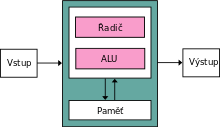
\includegraphics[width=8cm]{TVP_1_10_23@3.png}
    \end{figure}

\section{Harvardska architektura}
    \begin{itemize}
        \item{oddeluje fyzicky pameť programu a jejich spojovaci obvody}
        \item{nazev pochazi z prvniho pocitace vyuzivajici tuto architekturu Harvard Mark I; instrukce byly ulozeny na derovane pasce a data na elektromechanickych deskach}
        \item{CPU můze soucasne cist instrukci z programove pameti a pristupovat do pameti dat}
        \item{pouziva se ve specializovanych procesorech, obvykle v audio/video technice}
    \end{itemize}
    \subsection{Pameť}
        \begin{itemize}
            \item{neni treba mit pameť stejnych parametrů a vlastnosti}
            \item{dvoji pameť umozňuje paralelni pristup k obema pametim => vyssi rychlost zpracovani}
            \item{umisteni programu do ROM pameti můze zvysit bezpecnost systemu (program nelze modifikovat)}
        \end{itemize}
    \subsection{Rychlost}
        \begin{itemize}
            \item{rychlost procesorů se nekolikanasobne zvetsila o proti rychlosti hlavni pameti → tendence zredukovat pocet pristupů do hl. pameti.}
            \item{za vyssi cenu procesor můze byt mnohem rychlejsi}
            \item{pameť cache (vyrovnavaci) je velmi rychla; je ji mene nez hl. pameti; velikost cache je jeden z hlavnich aspektů urcovani rychlosti procesoru}
        \end{itemize}

\section{Sekvencni obvody}
    \begin{itemize}
        \item{nezavisi na okamzite hodnote vstupnich signalů ale i na poradi minulych vstupů}
        \item{jsou schopny uchovavat stav (obsahuji pameť); je potreba sledovat krome vstupnich promennych i vnitrni promenne}
        \item{delime na synchronni a asynchronni}
            \item[o] u asynchronnich se zmena vstupu promitne ihned do stavu obvodu
            \item[o] u synchronnich je zaveden synchronizacni signal (hodiny); zmena vstupu se promitne do obvodu az pri pulzu hodinoveho signalu
        \item{pameťova cast je tvorena kombinacnim obvodem - bistabilni klopny obvod; jeho úkol je uchovat informaci na vstupu i pote, co informace na vstupu jiz neni}
    \end{itemize}

\section{Kombinacni obvody}
    \begin{itemize}
        \item{vystup zavisi na okamzite kombinaci vstupů}
        \item{nemaji zadnou pameť}
        \item{zavislost vystupni funkce je popsana pravdivostni tabulkou nebo pomoci logickych vyrazů}
        \item{pro realizaci je mozne vyuzit}
            \item[o]{pevne pameti}
            \item[o]{zakladni logicke cleny (NAND; AND, NOR, OR, atd.)}
    \end{itemize}
    
\section{Bezpecnost}
    \begin{itemize}
        \item{obor zabyvajici se ochranou pocitacovych systemů a siti pred neopravnenym pristupem, kradezi nebo poskozenim hardwaru, softwaru. Hlavnim cilem je zajistit spolehlivost, integritu a soukromi údajů systemu.}
        \item{ochrana se da shrnou tremi kroky:}
            \item{prevence - ochrana pred hrozbami}[1)]
            \item{detekce - odhaleni neopravnenych cinnosti a slabych mist v systemu}[2)]
            \item{naprava - odstraneni slabych mist v systemu}[3)]
        \item{bezpecnost zahrnuje}
            \item[o]{omezeni fyzickeho pristupu k pocitaci a jeho zarizeni, ochrana pred neopravnenym manipulovani}
            \item[o]{umoznit pristup jen opravnenym osobam vyskolenym pro praci s pocitacem a daty}
            \item[o]{ochrana informaci pred kradezi, nelegalni tvorbou kopii}
            \item[o]{pouziti hardwarovych zarizeni vynucujici bezpecnostni opatreni}
            \item[o]{vyuziti mechanismů OS vynucujici chovani programů v souladu s pocitacovou bezpecnosti}
            \item[o]{omezeni mnozstvi programům, kterym je nutne důverovat}
            \item[o]{vyuziti zaznamů o zmenach v programech a systemech}
            \item[o]{vyuziti zabezpeceni operacniho systemu}
            \item[o]{vyuziti sifrovani pri komunikaci, praci s údaji a jejich prenosu}
            \item[o]{vyuziti bezpecneho ukladani a zalohovani}
            \item[o]{planovani reakce na incident}
    \end{itemize}

\section{Synchronizace}
    \subsection{vnejsich signalů}
        \begin{itemize}
            \item{proces, jenz ma za úkol usporadani signalů nebo casovych znacek pro komunikaci mezi různymi zarizenimi, systemy nebo procesy}
            \item{dosahuje se pomoci různych technik a zarizeni, jako jsou atomove hodiny, GPS, synchronizacni protokoly a specialni hardware}
            \item{zakladnim prvkem pro spravnou funkci modernich technologii a zarizeni}
        \end{itemize}
    \subsection{na úrovni procesů}
        \begin{itemize}
            \item{klicovy koncept v oblasti operacnich systemů a paralelniho programovani}
            \item{mechanismy a techniky slouzici k rizeni cinnosti různych procesů (nebo vlaken) v pocitacovem systemu}
            \item{cilem je zajistit efektivitu a bezpecnost procesů}
            \item{zakladni techniky synchronizace:}
                \item[o]{Race Conditions - nastavaji, kdyz vice procesů ma pristup ke sdilenym zdrojům (napriklad pameti) a snazi se je upravovat soucasne; můze vest k nepredvidatelnym chybam v datech}
                \item[o]{Mutual Exclusion - zakladni synchronizacni umozňujici procesům ziskat exkluzivni pristup k sdilenym zdrojům; jen jeden proces můze mit mutex v dany okamzik, coz eliminuje konflikty.}
        \end{itemize}
        
\section{Systemy s vice jadry}
    \begin{itemize}
        \item{jsou integrovane obvody se dvema nebo vice CPU jednotkami zvane jadro}
        \item{ridi se stejne jako systemy s jednim jadrem, az na fakt, ze vicejadrove systemy mohou spoustet procesy v jednotlivych jadrech → zvyseni rychlosti}
        \item{podpora vice jader je zavisla na programu a operacnim systemu}
        \item{pokud neni software napsan s podporou vice jader, program je nebude pouzivat}
    \end{itemize}
\end{document}
